\documentclass[12pt]{article}

% PACKAGES
\usepackage[margin = 1in]{geometry}
\usepackage{amsfonts}
\usepackage{amsmath}
\usepackage{amssymb}
\usepackage{multicol}
\usepackage{graphicx}
\usepackage{float}
\usepackage{xcolor}
\usepackage{amsthm}
\usepackage{dsfont}
\usepackage{hyperref}
\usepackage{setspace}
\usepackage{algorithm}
\usepackage{algpseudocode}

% MACROS
% Set Theory
\def\N{\mathbb{N}}
\def\R{\mathbb{R}}
\def\C{\mathbb{C}}
\def\Z{\mathbb{Z}}
%\def\^{\hat}
\def\-{\vec}
\def\d{\partial}
\def\!{\boldsymbol}
\def\X{\times}
%\def\-{\bar}
\def\bf{\textbf}
\def\l{\left}
\def\r{\right}
\def\~{\tilde}
\date{August 2022}
\doublespacing
\begin{document}

\begin{titlepage}
    \begin{center}
        \vspace*{1cm}
            
        \Huge
        \textbf{Multifidelity Finite Basis Physics Informed Neural Networks}
            
            
        \vfill
            
        
        Name: Damien Beecroft\\
        Hosting Site: Pacific Northwest National Lab\\
        Mentors: Amanda Howard and Panos Stinis\\
        \vspace{2cm}
        \begin{flushleft}
       	Mentor's Signature:\\
       	\end{flushleft}
       	\Large
        
            
    \end{center}
\end{titlepage}

\section*{Abstract}
\begin{singlespace}
Physics informed neural networks (PINNs) struggle to successfully learn solutions to differential equations that exhibit high-frequency oscillations or multi-scale behavior. Multilevel finite basis physics informed neural networks (FBPINNs) tackle this problem by recursively discretizing the solution domain and training coupled neural networks on the subdomains. In this work we integrate multifidelity methods into multilevel FBPINNs to improve convergence. We tested this method on a collection of test problems and analyzed the errors and solution structure to determine the quality of the results. This project can benefit anyone that is trying to model a differential equation that classical numerical or analytical methods struggle to solve.
\end{singlespace}
\vspace{1cm}
\begin{figure}[H]
\center
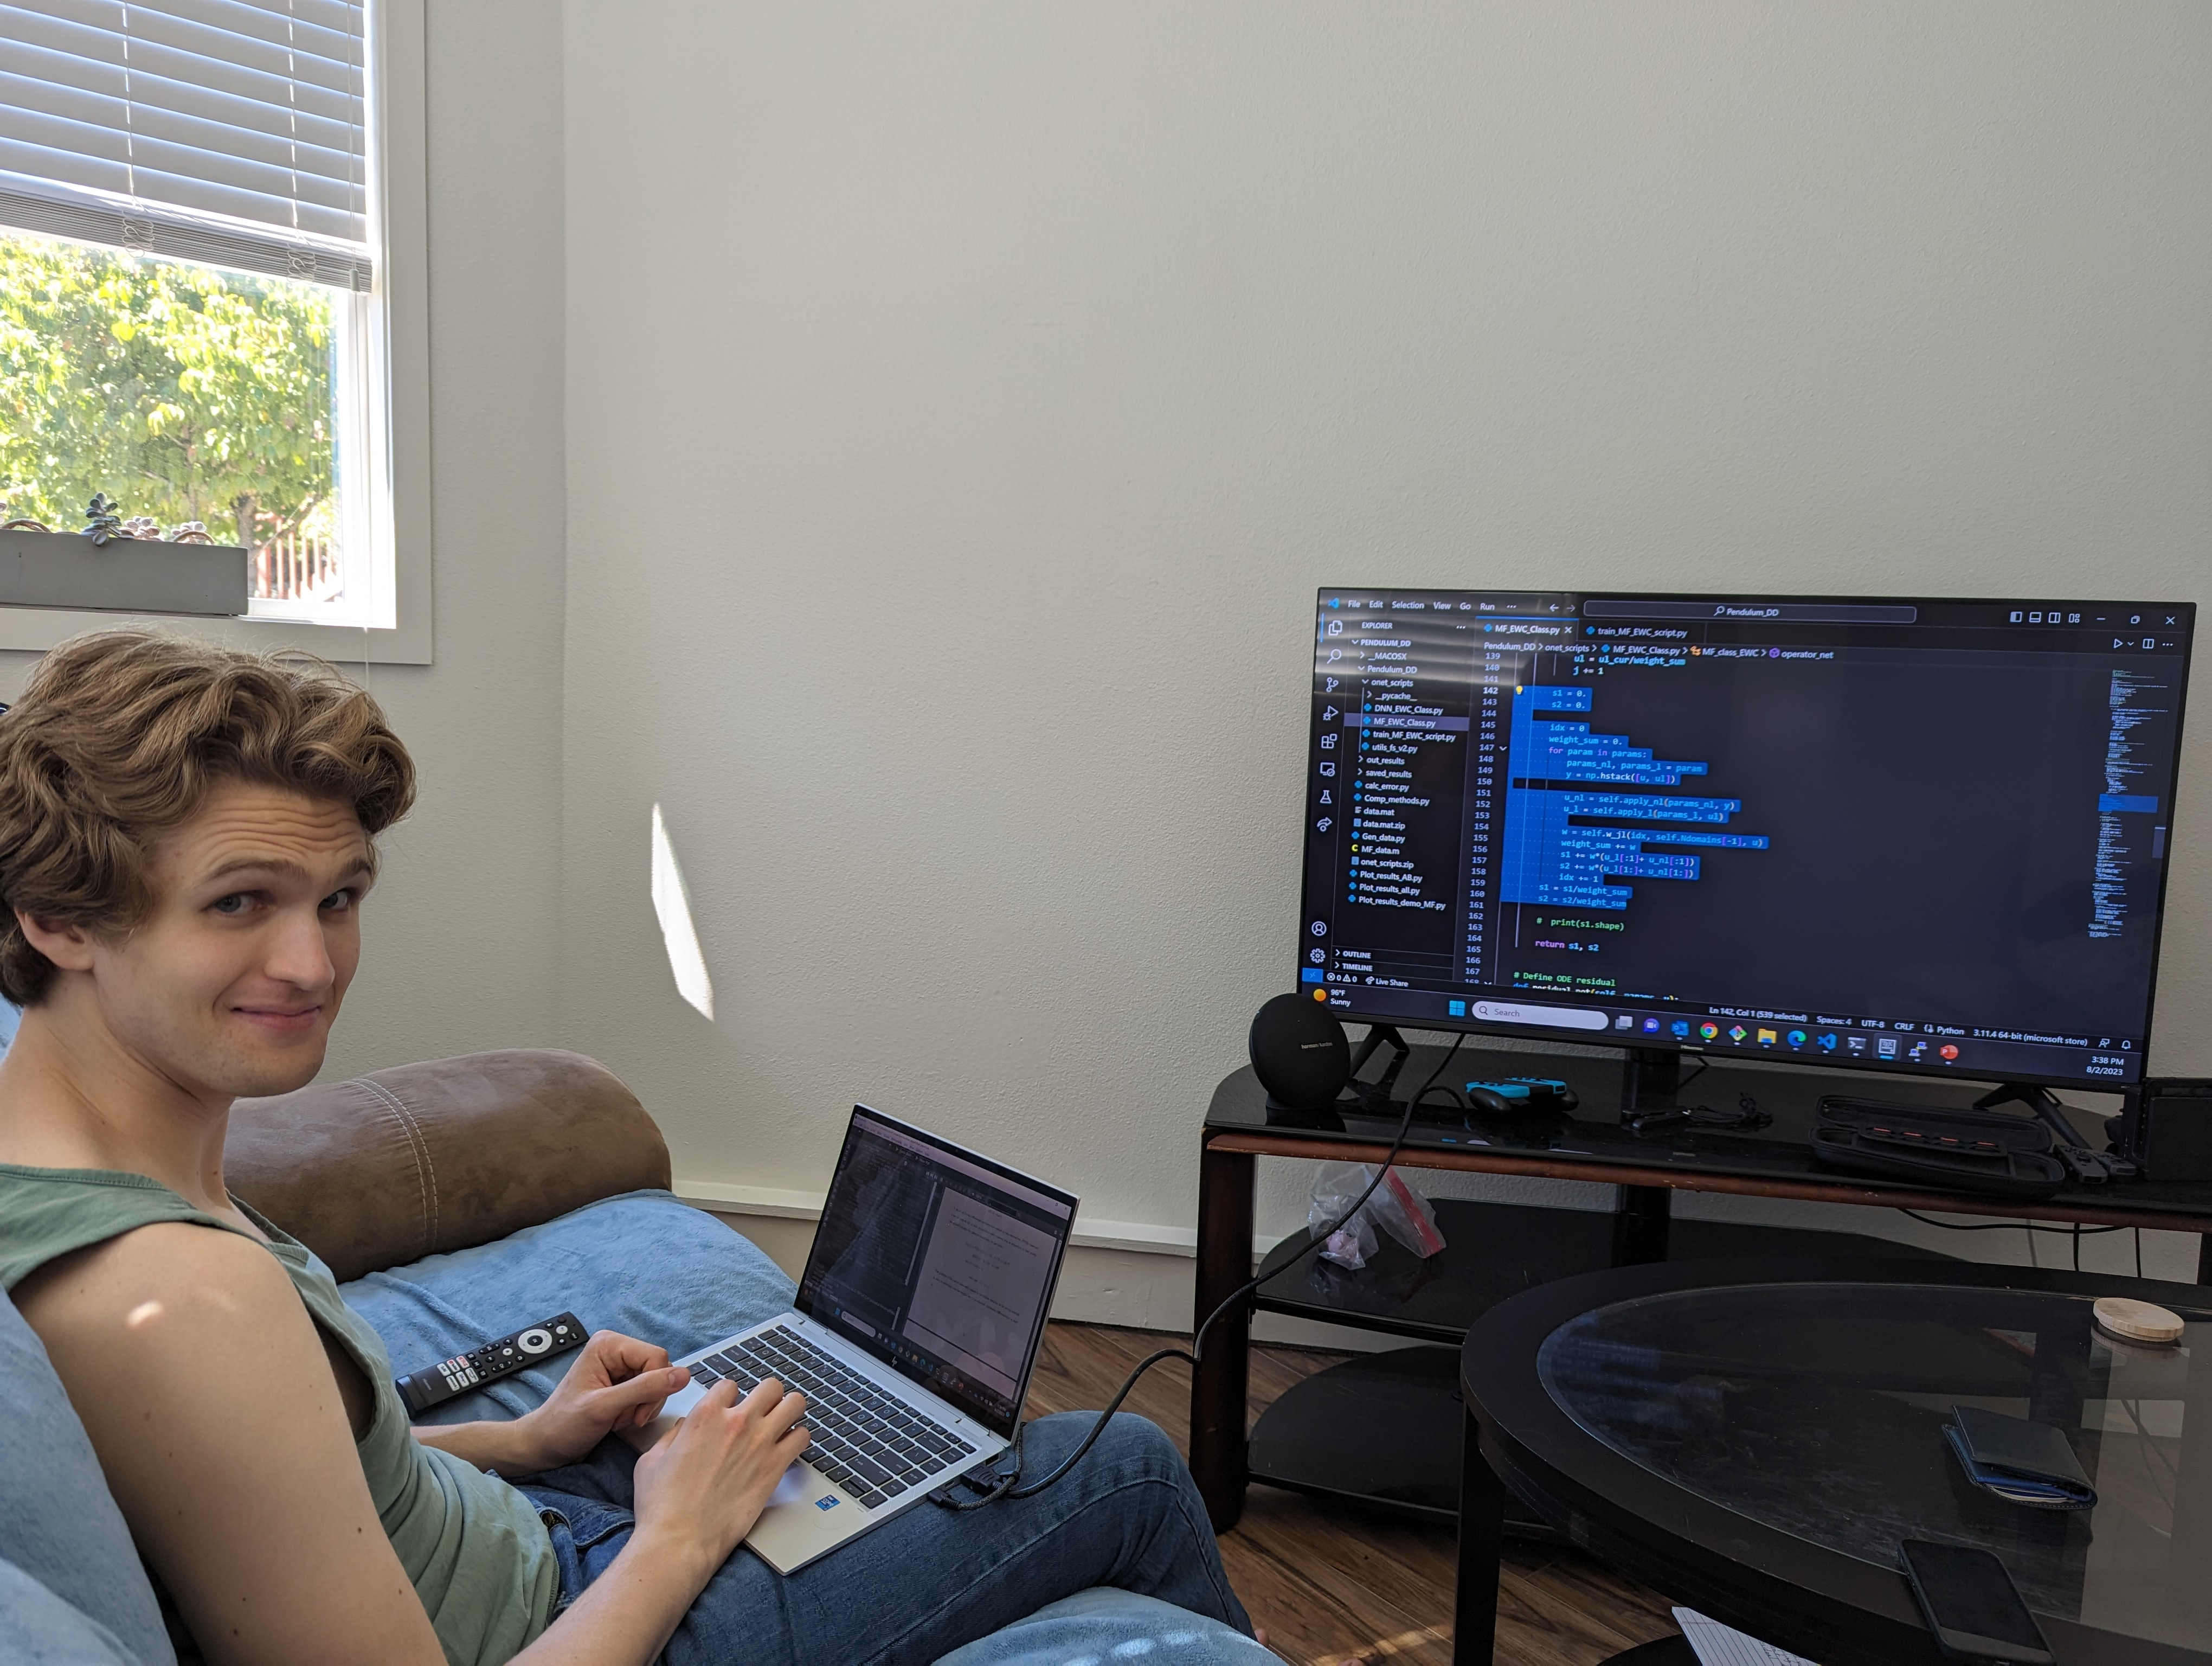
\includegraphics[width = 0.9\textwidth]{imgs/me.jpg}
\caption{My internship at Pacific Northwest National Lab was virtual. My office was anywhere I lugged my computer. On some of my more adventurous days I ventured all the way down to my living room to use the television as a secondary monitor. On an even more auspicious occasion my girlfriend and soon to be doctor Caitlin Neher was kind enough to take my photo for this final report.}
\label{fig:me}
\end{figure} 

\vfill
\newpage
\section{Introduction}

Physics informed neural networks (PINNs) learn the solution to a differential equation for a given set of initial and boundary conditions \cite{pinns}. We briefly review PINNs here. Suppose that we have the following differential equation.
\begin{align} 
	u(t,x)_t + N[u(t,x)] &= 0 \quad \text{for} \quad x \in \Omega, \: t \in [0,T] \notag\\
	B[u(t,x)] &= 0 \quad \text{for} \quad x \in \partial \Omega\\
	u(0,x) &= u_0(x) \notag
\end{align} \label{eq:dq}
$N$ and $B$ are known differential operators that contain no time derivatives. PINNs construct a neural network $\~u(t,x)$ that, is penalized every training step in proportion to how poorly the network satisfies the physical constraints.
\begin{align}
	\~u(t,x)_t + N[\~u(t,x)] &= l_1 \quad \text{for} \quad x \in \Omega, \: t \in [0,T] \notag \\
	B[\~u(t,x)] &= l_2 \quad \text{for} \quad x \in \partial \Omega\\
	\~u(0,x) - u_0(x)& = l_3 \notag \\
	\text{total loss}& = l_1 + l_2 + l_3 \notag
\end{align} \label{eq:loss}
\noindent The gradient of the total loss is taken with respect to the hidden variables of the neural network to determine how the weights are to be adjusted. Automatic differentiation is used to differentiate the neural network with respect to the temporal and spatial variables. 
\par This is a simple and elegant framework. However, PINNs struggle to learn oscillatory and multi-scale solutions. They often converge to erroneous fixed point solutions in these scenarios \cite{fixedpts}. This makes sense since fixed point solutions have a small residual and small hidden weights. There are a variety of methods and techniques that have been introduced to improve the convergence of PINNs. 
%Please refer to the glossary at the end for readings on some of these techniques. \textcolor{red}{MAKE GLOSSARY} 
\section{Description of Project}
\par My research this summer focused on testing a new extension of PINNs: multifidelity finite basis physics informed neural networks (MFFBPINNs). This method is the combination of two other extensions of PINNs: multifidelity PINNs and multilevel finite basis PINNs.
\par Multifidelity PINNs learn from two separate data sources: a high and low fidelity data source. The multifidelity network learns the correlation between the two data sources to achieve an accurate prediction of the true solution \cite{mfpinns}. This process is illustrated in Figure \ref{fig:mfpinn}.

\begin{figure}[h]
\center
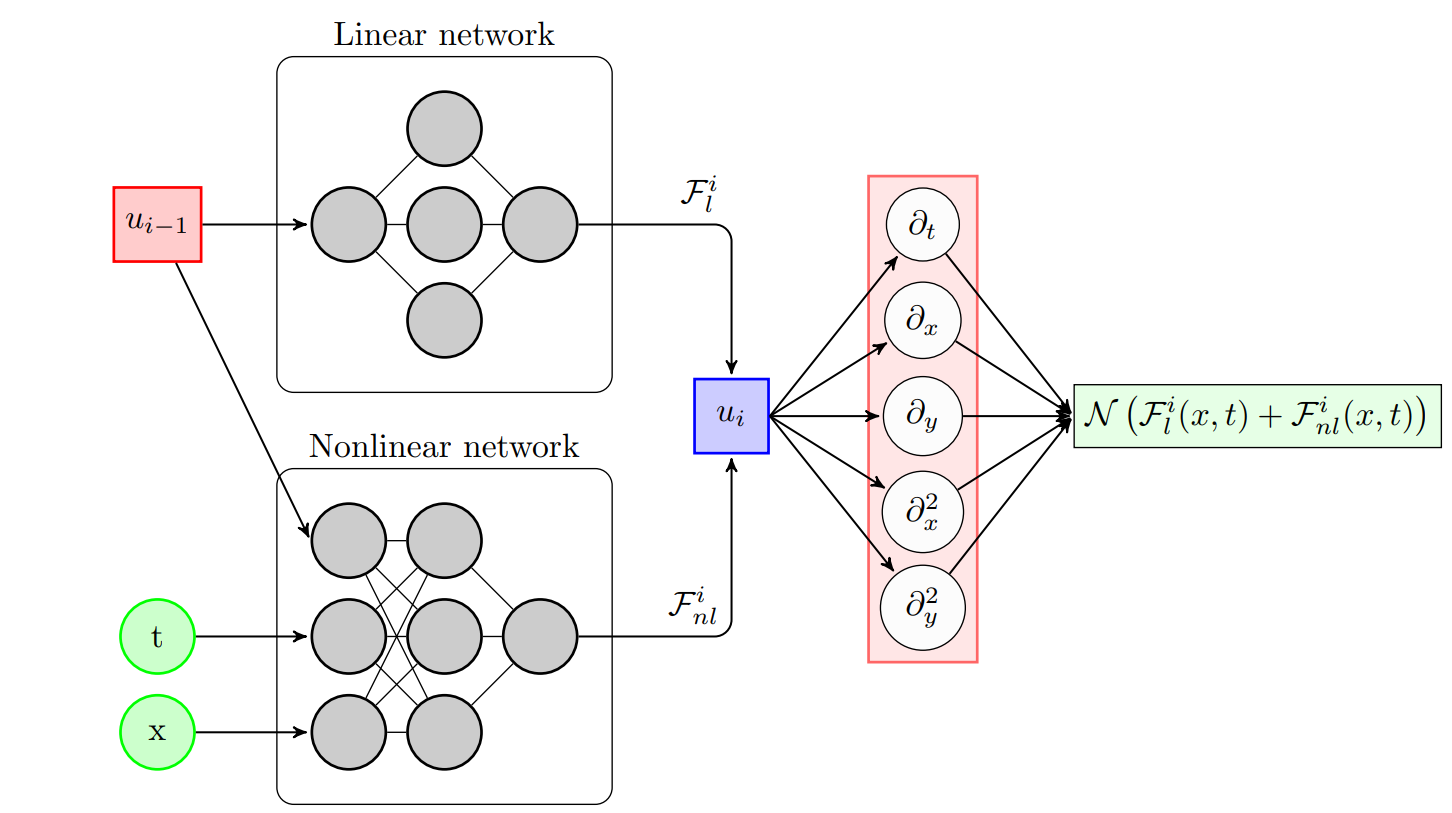
\includegraphics[width = 0.7\textwidth]{imgs/mfpinns2}
\caption{This is a graphic of a multifidelity PINN from Meng at al. \cite{mfpinns}. The multifidelity PINN takes in the low fidelity approximations ($u_{i-1}$) and the collocation points ($x$, $t$) and outputs a new set of approximations ($u_i$). This network can then be differentiated to see how well it satisfies the differential equation.}
\label{fig:mfpinn}
\end{figure} 

\par Multilevel finite basis PINNs take the problem domain and decompose it into a hierarchy of overlapping subdomains \cite{fbpinns}. A neural network is trained on each of these subdomains and the levels are averaged to get the overall solution. This process is illustrated in Figure \ref{fig:fbpinn}.

\begin{figure}[t]
\center
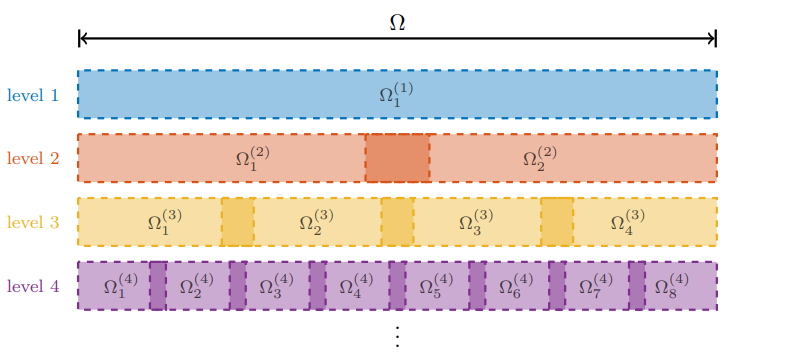
\includegraphics[width = 0.7\textwidth]{imgs/domain_decomp2}
\caption{This is a graphic illustrating multilevel finite basis PINNs from Dolean et al. \cite{fbpinns}. Level 1 is trained first. Then, level 2 is trained to correct for the residual of level 1. Levels 1 and 2 are averaged to get the new estimate of the global solution. Level 3 is trained to correct for the errors of the new global solution. Levels 1, 2, and 3 are averaged. This process continues until a desired level of accuracy is achieved.}
\label{fig:fbpinn}
\end{figure} 

\par Now we can introduce MFFBPINNs. Suppose we are attempting to learn the differential equation posed in Equation \ref{eq:dq}. MFFBPINNs construct a hierarchy of neural networks. On the zeroth level of the hierarchy is a single fidelity neural network that requires no low fidelity data to make a prediction. This single fidelity method could be a classical PINN or even the solution of a numerical solver. The only caveat is that we need to be able to take spatial and temporal derivatives of this single fidelity solution. After the single fidelity network is trained on $\Omega$, the domain is broken up into a set of overlapping subdomains for the first multifidelity level: $\{\Omega^1_n\}_{n=0}^{N_1}$. Each multifidelity PINN on this level takes in the evaluation of the single fidelity PINN on the zeroth level as its low fidelity approximation to the solution. Now, the multifidelity PINNs on the first level are trained while the single fidelity network's parameters are frozen. For the second level of multifidelity PINNs the process is repeated. The domain is broken up into a new set of subdomains: $\{\Omega^2_n\}_{n=0}^{N_2}$. However, now the multifidelity networks on the first level provide the low fidelity data for the second level. This process repeats until a desired accuracy is achieved. This process is illustrated in Figure \ref{fig:mffbpinn}.

\begin{figure}
\centering
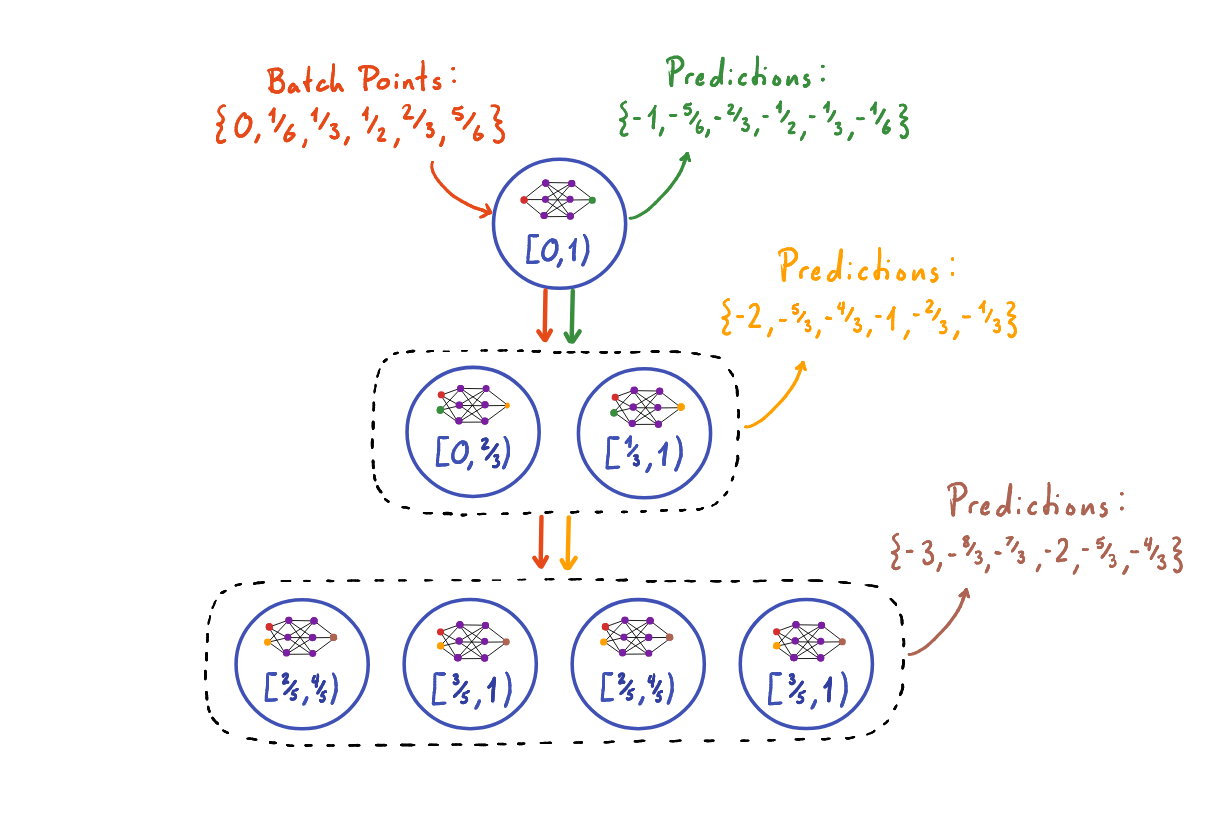
\includegraphics[width=0.8\textwidth]{imgs/mffbpinn}
\caption{A simple diagram of the MFFBPINN algorithm for a 1D problem where the number of domains is doubled at each step.}
\label{fig:mffbpinn}
\end{figure}

\section{Contributions Made to the Project}
I had two tasks to accomplish during this project. The first was to create an efficient implementation of the MFFBPINN algorithm. The second was to test the MFFBPINNs on a collection of test problems. This position was ten weeks. I spent roughly the first three weeks reading up on the PINNs, setting up my computer, learning to use the PNNL GPU cluster, and trying to understand source code that Amanda sent me. I began my attempt to improve on Amanda's source code on week four. She had a rather ad hoc implementation of the MFFBPINN algorithm set up for a damped pendulum equations. I call this code "ad hoc" because every neural network on every subdomain was evaluated on the entire domain. However, only the points inside the domain of the neural network have a non-zero weight. Therefore, many points were evaluated by the network only to be zeroed out by the weight function later on. This is very inefficient. I began developing an algorithm that fixed this problem and was also very flexible so that one could generalize the implementation to higher dimensions with more complex subdomains. I spent weeks four and part of week five doing this. Towards the end of the fifth week I began trying to integrate Jax into my method. This did not work. Jax is very efficient at the cost of flexibility. I could not figure out how to integrate Jax into my algorithm. I tried for roughly a week and a half to no avail. At this point Amanda and Panos said that I should prioritize getting results over finishing the algorithm. Thus, I used the "ad hoc" pendulum code to produce results. The code struggled to converge for this problem, so I had to play around with parameters to get good results. I also implemented the causality weighting from Wang et al. \cite{causality}. I also had to implement the domain decomposition for the wave and Allen-Cahn equations. I used this code to produce the following results. \textcolor{red}{ADD SOME RESULTS}

\section{New Skills and Knowledge}
I gained a great deal of knowledge during the course of this internship. I began the internship by reading papers on PINNs and different methods for overcoming their convergence issues. After I had gained a sufficient basis of knowledge on PINNs I began setting up my account on the PNNL GPU cluster: Marianas. Setting up and using this account forced me to brush up my skills in a variety of tools including Anaconda, Bash, Slurm, and GitHub. After I had set up my account on the cluster I began working on implementing  MFFBPINNs to solve a variety of test problems: damped pendulum, wave equation, and Allen-Cahn equation. Working on the MFFBPINN implementation extended my knowledge of Python and introduced me to Jax. Furthermore, I did not have much hands on experience training neural networks prior to this internship. This summer has given me the opportunity to put theory into practice and vastly expand my knowledge in the field of machine learning.

\section{Experience and Impact on My Career}
Machine learning is by far the hottest research topic currently. There are many research positions in this area. Until now I was not certain what these positions would be like on a day to day basis. My internship at PNNL has given me valuable insight on this matter and will enable me to make a more informed decisions concerning my career path.

\section{Relevance to the Mission of NSF}
The statutory mission of NSF is, "To promote the progress of science; to advance national health, prosperity, and welfare; and to secure the national defense; and for other purposes." The methods being developed in this work may one day help engineers and scientists solve challenging differential equations without expertise in analytical or numerical methods. This could in turn accelerate the development and production of technologies for the benefit of humanity.

\section{Acknowledgements}
I acknowledge and appreciate the support from the National Science Foundation Mathematical Sciences Graduate Internship program. This project was completed with support from the U.S. Department of Energy, Advanced Scientific Computing Research program, under the Scalable, Efficient and Accelerated Causal Reasoning Operators, Graphs and Spikes for Earth and Embedded Systems (SEA-CROGS) project (Project No. 80278), The computational work was performed using PNNL Institutional Computing at Pacific Northwest National Laboratory. Pacific Northwest National Laboratory (PNNL) is a multi-program national laboratory operated for the U.S. Department of Energy (DOE) by Battelle Memorial Institute under Contract No. DE-AC05-76RL01830.
\bibliographystyle{plain}
\bibliography{refs}
\end{document}

%During the course of this internship, we developed two main ways to implement this algorithm. Each one is centered around how batching is done. In the first implementation, a batch containing points in the entire domain $\Omega$ is sent to the MFFBPINN. In this construction we use a tree of neural networks. The zeroth level creates its solution prediction. The networks on the first level (which are all children of the single fidelity network on the zeroth level) then look at the points in the original batch and the low fidelity solution from the zeroth layer and make their own approximation for the points that are within their subdomains. The child of each network in the second level then take in the batch points and approximations of their parents and create new approximations on the points in their subdomains and so on and so forth. A diagram illustrating this process is given in figure \ref{fig:batch1}. This method scales well with higher dimension and is rather flexible with respect to the shape of the subdomains.

%In the second implementation of the MFFBPINN, distinct batches of residual points are created for each intersection of the subdomains on the highest level. These batch points are then fed down to the neural networks on the lower levels to get the low fidelity approximations. This method is illustrated in Figure
